% !TEX encoding = UTF-8 Unicode

\documentclass[twocolumn,10pt,a4j]{jsarticle}
\usepackage{kougai}


\title{ケプストラム法を用いた反射音除去の一提案}
\author{1632038 岡田 秀  指導教員 須田 宇宙 准教授}
\date{}

\begin{document}

\maketitle

\section{はじめに}
%1章には,背景・問題点・目的を順番に書く.
%背景は,広く一般的な事柄を書いて,読む人に同意を抱かせつつ問題点につなぐ.
%問題点では,「〜という問題点がある」などのように,「問題」または「問題点」と言う単語を用いて,目的につなぐ.
%目的では,「そこで本研究では」から始めて,「〜を目的とする」で締める.
%以下は過去の卒業研究最終審査用の梗概の抜粋である.

%背景+問題点
日本は災害が多い国であり,非常放送は重要性が高い\cite{oka1}.スピーカから離れている地点で放送を聞くと物体による反射音で内容を聞き取りづらいことが多い.信号処理によって反射音を除去できれば,放送内容を聞き取りやすくなる.

反射音を除去する方法として佐藤\cite{oka1}の研究では非常用放送の音声の先頭に信号音を付加させた.その信号音を基準とし,他のデバイスによってリアルタイムにインパルス応答を計算し,反射音を除去する手法を提案している.


%目的
本研究では,逆畳込みとケプストラム法を用いて残響音を除去し非常放送を明瞭に聞き取ることを目的とする.

\section{残響とインパルス応答}

室内などの閉空間内で発生した音は壁にあたって反射する.反射した音は壁に当たることを繰り返し,1回の反射ごとにエネルギーを失いながら,次第に減少していく.このような多重の反射が作り出す減少を残響という.
音源から単一の衝撃音を発したときの受音点での音の観測結果は例として図1のようになる.直接音をインパルスと呼び,それに対する空間情報すべてをインパルス応答と呼ぶ\cite{oka2}.


\begin{figure}[h]
\begin{center}
 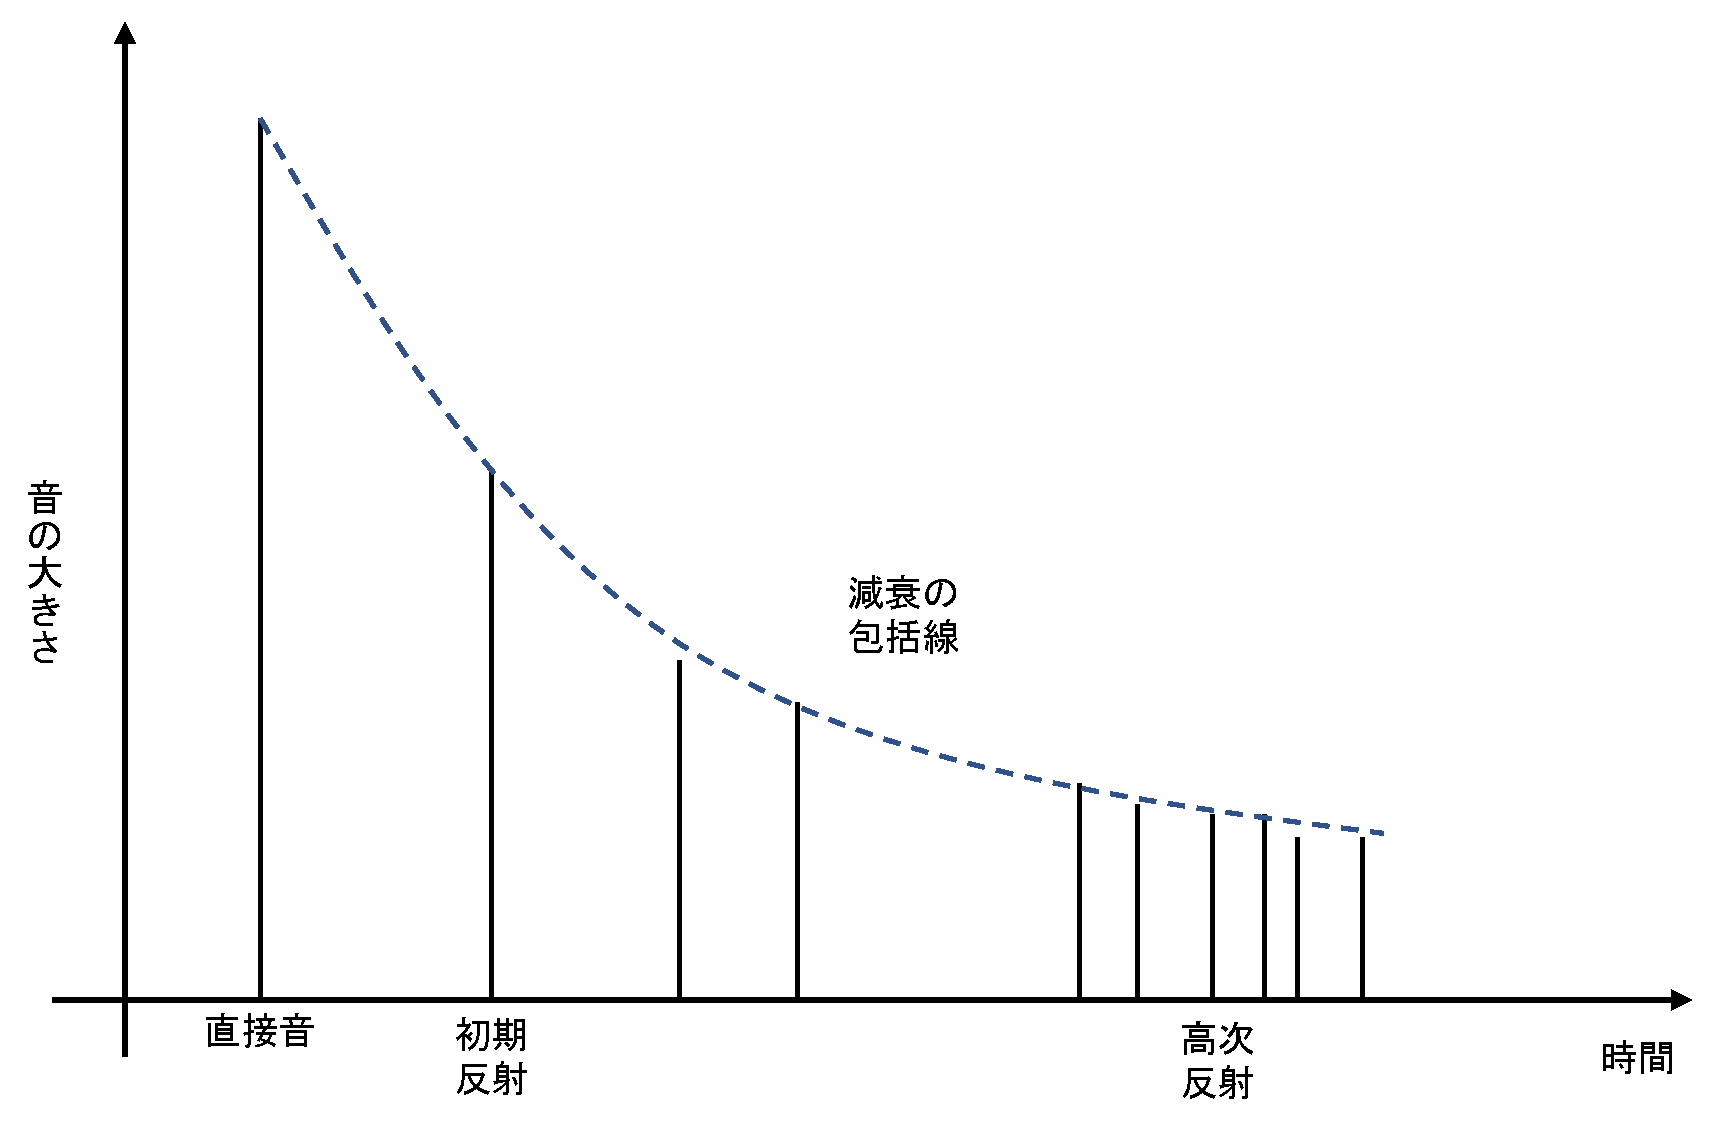
\includegraphics[clip,width=70mm,height=32mm]{ReverberationImpulseResponse.pdf}
\end{center}
 \caption{インパルス応答の例\cite{oka2}}
 \label{fig:教科書}
\end{figure}



%2章では,研究テーマとして取り上げた内容(この例では「電子教科書」についての研究だった)について説明する.
%その他,数式を用いて理論を説明することも可能である.

%シミュレータ教材を利用する際には,シミュレートを行っている現象そのものについての理解を促す必要がある.
%そのためには,シミュレーションの解説や教材の操作方法などを確認しながら利用することが,より効果的であると考えた.
%この考えに基づいて制作した電子教科書の一部を図\ref{fig:教科書}に示す.
%左側には,シミュレータに関する前提知識や解説を記述した.
%右側には教材の操作方法を記述し,それを確認しながらシミュレータ教材を利用することを可能とした.
%電子教科書にはシミュレータ教材を6つ搭載し,全体で30ページほどの教科書を制作した.
%一方,電子書籍の標準的フォーマットであるePub形式の電子書籍を閲覧できるリーダは限られている上,動作が安定しないことがある.
%その中で,iPadに標準搭載されePub形式を閲覧可能であるiBooksを,本研究で利用するリーダとした.
%そのためシミュレータ教材を搭載後,機能の動作確認はiBooksで行った.
%iBooksではグラフ描画やアニメーションは可能であるが,音源再生や音声入力は実行できないことを確認した.%(できる気がしてきた)

%\begin{figure}[h]
%\begin{center}
% \includegraphics[clip,width=85mm,height=55mm]{textbook.pdf}
%\end{center}
% \caption{電子教科書サンプル}
 %\label{fig:教科書}
%\end{figure}


\section{提案手法}
本研究では,反射音が直接音に畳み込まれていると考えた.そのため反射音が付加した音声を元信号で逆畳み込みをすることで反射音を求められると考えた.また,反射音が付加されている音声から反射音を除去するために信号同士の計算が簡単になるケプストラム法を用いて反射音の除去された信号の抽出が可能である.
逆畳み込みによって求められた反射音D(t),反射音が含まれた信号音R(t),放送内容の先頭に付加された信号音
S(t)とすると以下のように表すことができる.
\begin{comment}

\begin{eqnarray}
  D(f) = \mathcal{F}[D(t)]\\
  g(f) = |D(f)|^2\\
  b(f) = \log g(f)\\
  R(f) = \mathcal{F}[R(t)]\\
  g'(f) = |R(f)|^2\\
  a(f) = \log g'(f)\\
  d(f) = a(f) - b(f)\\
  h(f) = e^d(f)\\
  S(t) = \mathcal{F}^{-1}[h(f)]
\end{eqnarray}

\end{comment}


\begin{figure}[h]
\begin{center}
 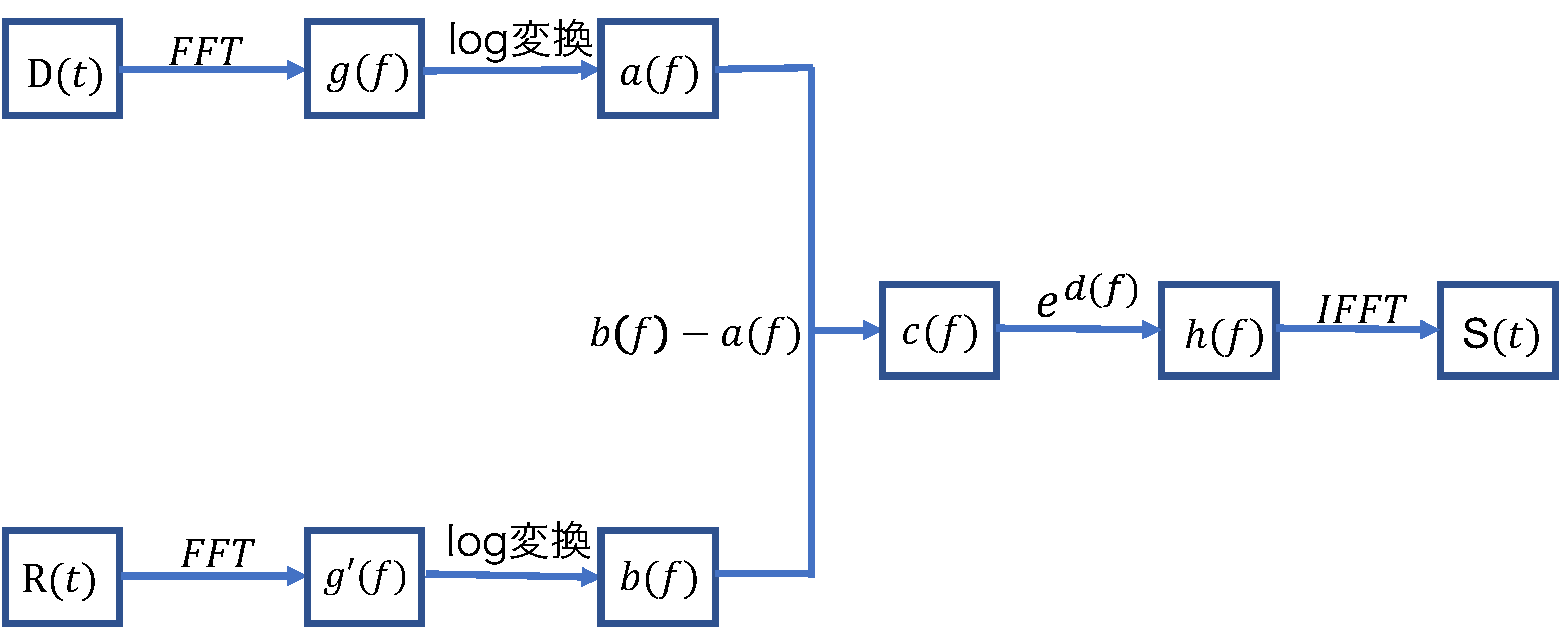
\includegraphics[clip,width=65mm,height=22mm]{flokougai.pdf}
\end{center}
 \caption{ケプストラム法理論}
 \label{fig:教科書}
\end{figure}

\begin{figure}[h]
\begin{center}
 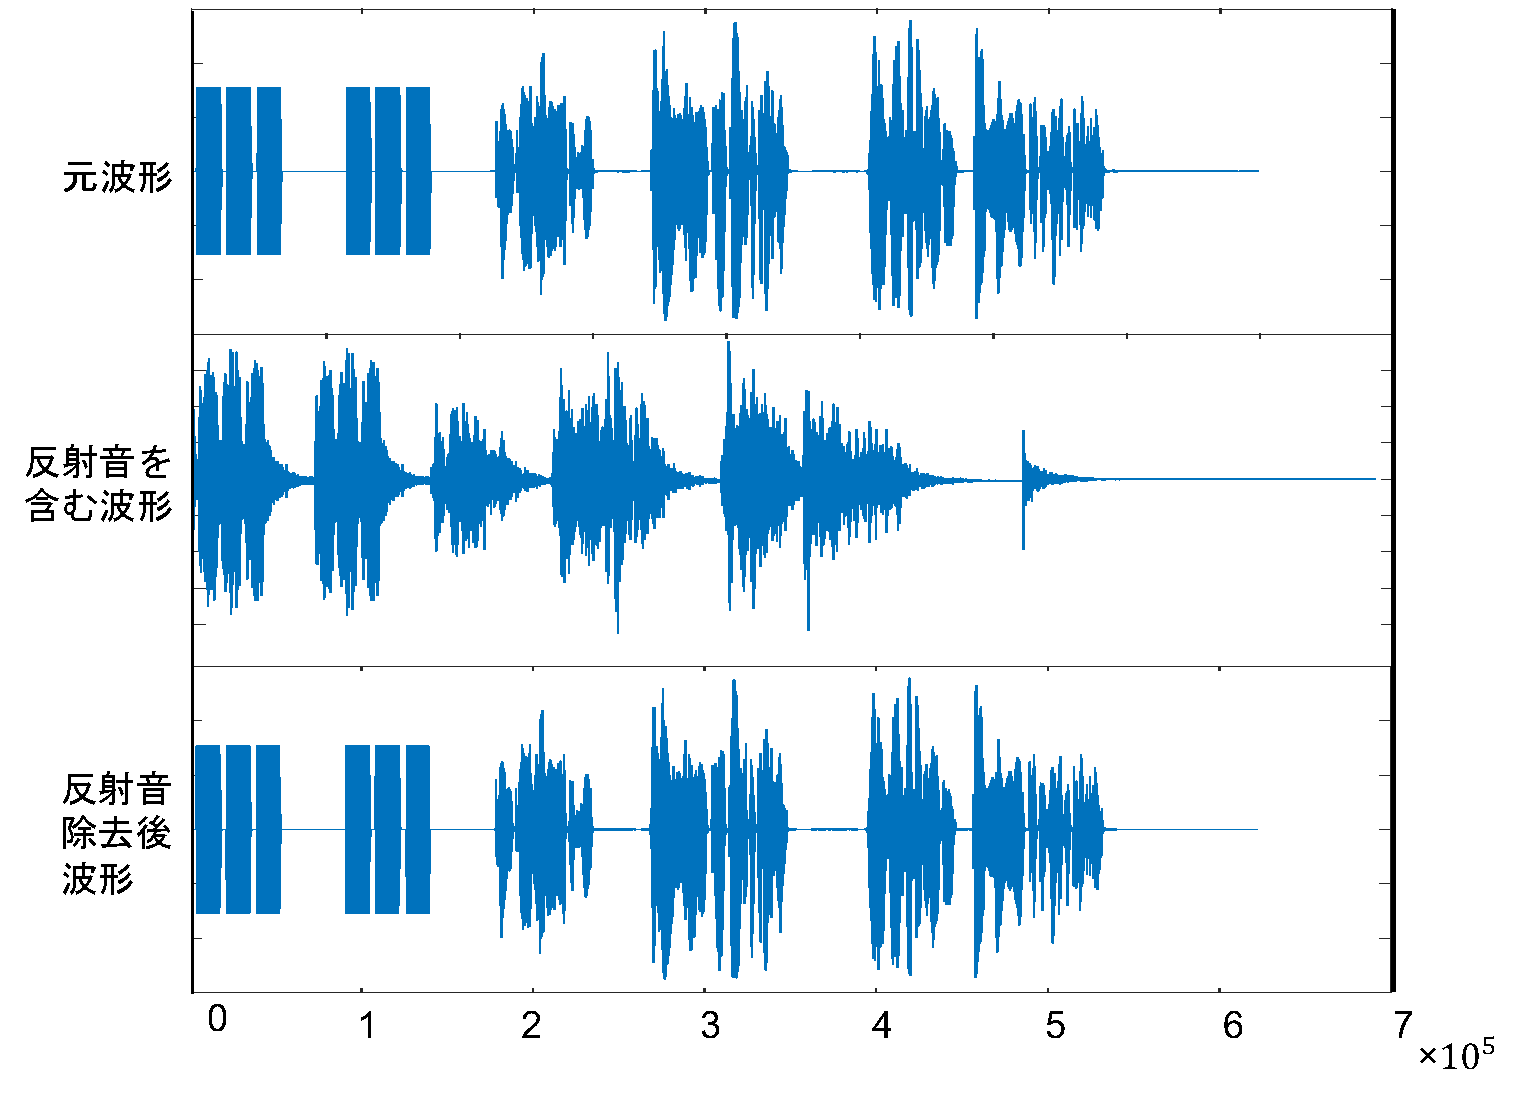
\includegraphics[clip,width=70mm,height=45mm]{kekkahakei.pdf}
\end{center}
 \caption{反射音除去結果}
 \label{fig:教科書}
\end{figure}


%3章には,中間審査用の梗概では実際に行う作業について(図を用いて)説明する.
%最終審査用の梗概では,やったことを示す.
%コンテンツを作成した場合にはコンテンツのスクリーンショットなどを用いる.
%調査が主であれば,調査の概要と結果のグラフなどを使用する.

%この文章では1章が長すぎるので,見た目のバランスが悪い.
%通常の梗概の割合は左側に1章と2章,右側に3章と4章のように並ぶ.
%もちろん多少の前後は有るので,きっちりと合わせなくても良い.

%通常,図は2枚程度である.
%図1枚+表1面でも構わない.
%梗概を書き始める前に,使用する図を決めてからレイアウトしていくと雰囲気がつかみやすくて良い.

\section{評価実験とその結果}
本研究の評価実験では,反射音の付加した音声とその波形から反射音を除去した音声を用いた.自然災害時に流れると考えられる,地震発生時や津波時の避難を促す文章など最長18秒,最短6秒の文章を用いた.これを各4編
計8編用意した,被験者には反射音付きの音声2編と除去後の音声2編の計4編を聞いてもらった上で,内容を書き出してもらいその正答率を調べた.その結果を図3に示す.
\begin{figure}[h]
\begin{center}
 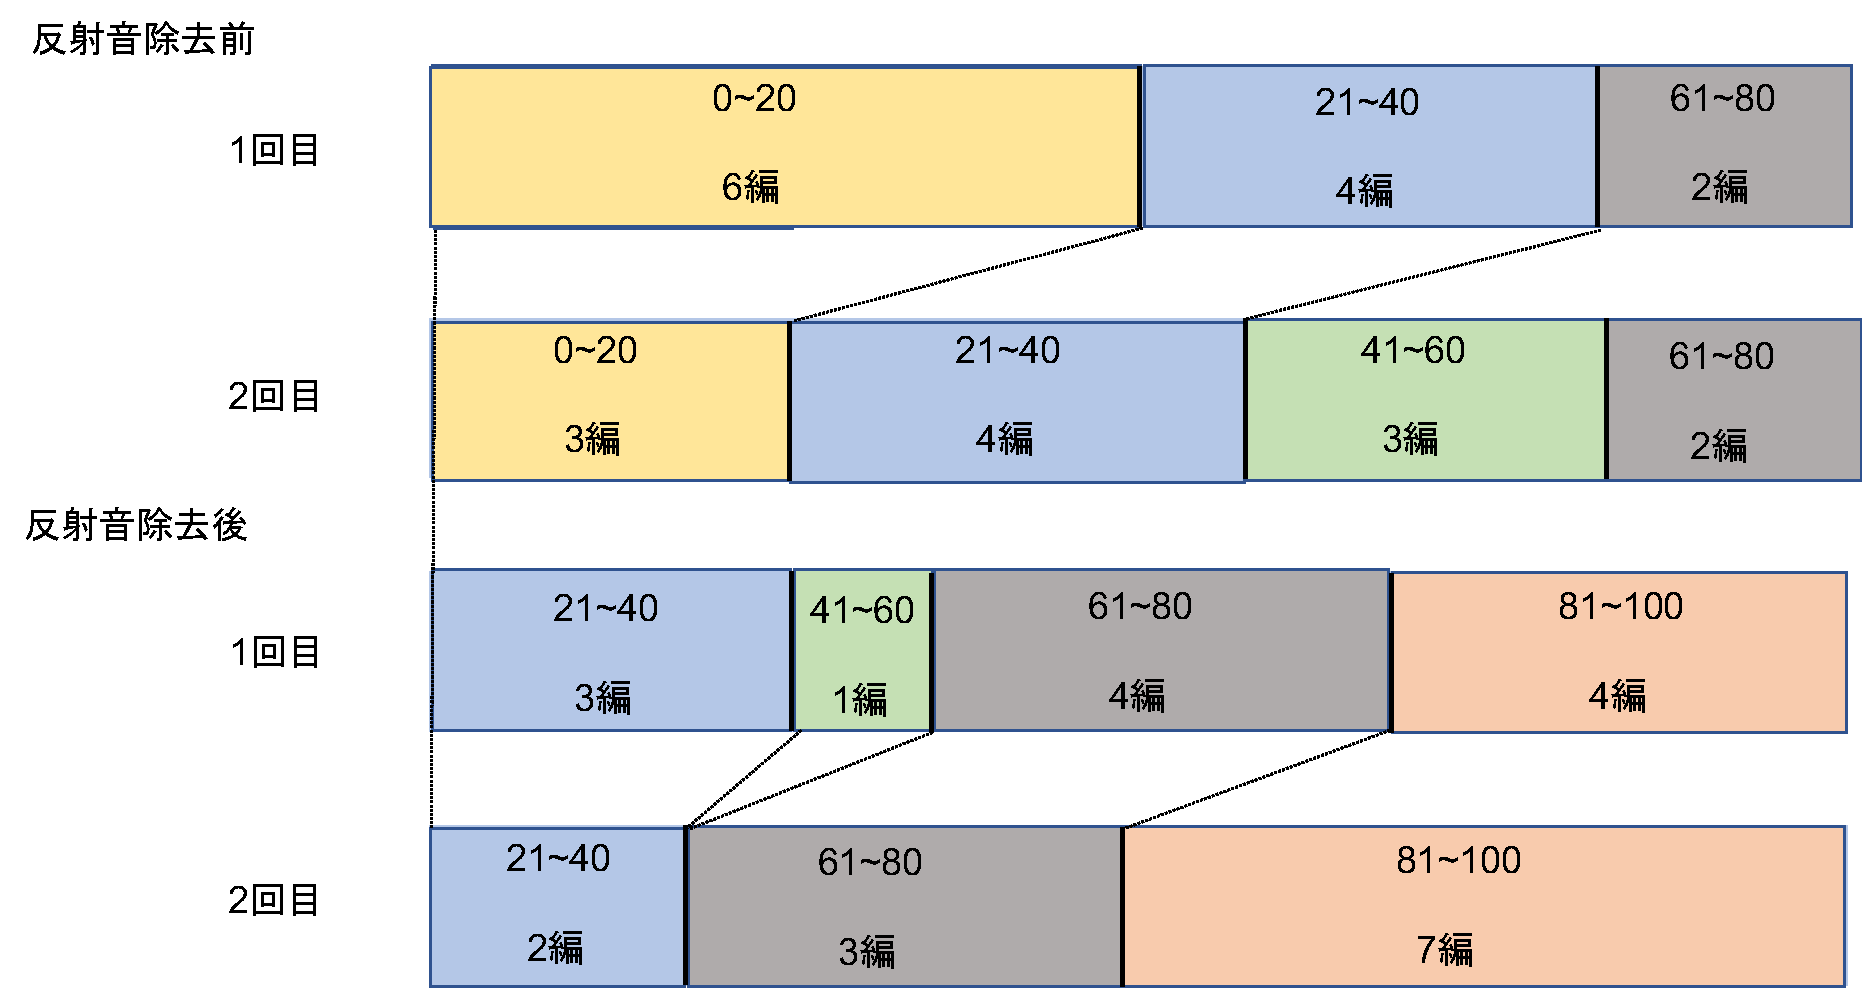
\includegraphics[clip,width=70mm,height=40mm]{shitsumon.pdf}
\end{center}
 \caption{実験結果}
 \label{fig:教科書}
\end{figure}
加えて行った放送内容が理解できたかという問いに対しても反射音を付加している音声より除去後の音声のほうが内容を理解して聞き取れていることがわかる.

\section{おわりに}
%中間審査用の梗概では4章のタイトルとして「今後の予定」,最終審査用5の梗概では「おわりに」などを用いる.
%たいてい2〜3行程度でまとめる.


本研究では先行研究\cite{oka2}をもとに逆畳込みとケプストラム法を用いることで反射音の除去を行った.評価実験を行い,反射音のある音声よりも除去された音声が聞き取りやすいことを確認した.今後,災害の現場で反射音除去の技術が活かされることが期待される.
\begin{thebibliography}{99}
\bibitem{oka1}国土技術センター,"自然災害の多い国",http://www.jice.or.jp/knowledge/japan/commentary09
\bibitem{oka2}佐藤 由希子,"インパルス応答を用いた反射音除去のための一提案", 千葉工業大学卒業論文, 2014
\bibitem{oka3}小泉 宣夫,"基礎音響・オーディオ学",コロナ社 2005 36-38頁
%\bibitem{oka2}米原市公式ウェブサイト ベルホール310舞台断面図http://www.city.maibara.lg.jp/0000002315.html

\end{thebibliography}
\end{document}
